\documentclass[tikz]{standalone}

\colorlet{FilledSurface}{blue!20}
\colorlet{FilledSurfaceGroupOne}{blue!20}
\colorlet{FilledSurfaceGroupTwo}{red!20}
\colorlet{FilledSurfaceGroupThree}{green!20}
\colorlet{FilledSurfaceGroupFour}{magenta!20}
\colorlet{FormulaBackground}{green!10}
\colorlet{FormulaFrame}{green}


\usetikzlibrary{calc, arrows.meta, angles}

\begin{document}
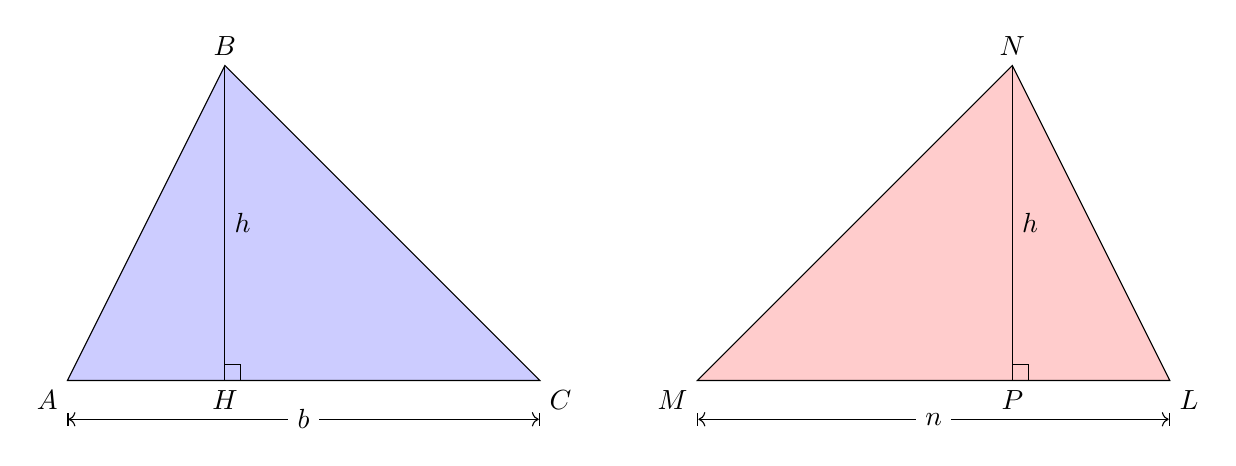
\begin{tikzpicture}

    \coordinate (A) at (0,0);
    \coordinate (B) at (2,4);
    \coordinate (C) at (6,0);

    \coordinate (M) at (8,0);
    \coordinate (N) at (12,4);
    \coordinate (L) at (14,0);

    \draw [fill=FilledSurfaceGroupOne] (A) node [below left]{$A$}
    -- (B) node [above]{$B$}
    -- (C) node [below right]{$C$}
    -- cycle;

    \draw [fill=FilledSurfaceGroupTwo] (M) node [below left]{$M$}
    -- (N) node [above]{$N$}
    -- (L) node [below right]{$L$}
    -- cycle;

    % Dibujar longitud de las bases
    \draw[color = black,|<->|] ($(A)!14pt!-90:(C)$) to node [fill=white, midway] {$b$} ($(C)!14pt!90:(A)$);
    \draw[color = black,|<->|] ($(M)!14pt!-90:(L)$) to node [fill=white, midway] {$n$} ($(L)!14pt!90:(M)$);

    % Dibujar longitud de las alturas
    \coordinate (Bproj) at (B |- A);
    \draw (B) -- node [right] {$h$} (Bproj) node [below] {$H$};
    \path pic [draw,angle radius=2mm] {right angle = B--Bproj--C};

    \coordinate (Nproj) at (N |- M);
    \draw (N) -- node [right] {$h$} (Nproj) node [below] {$P$};
    \path pic [draw,angle radius=2mm] {right angle = N--Nproj--L};

\end{tikzpicture}
\end{document}
